\strut \vspace{20pt}

\begin{figure}
    \centering
    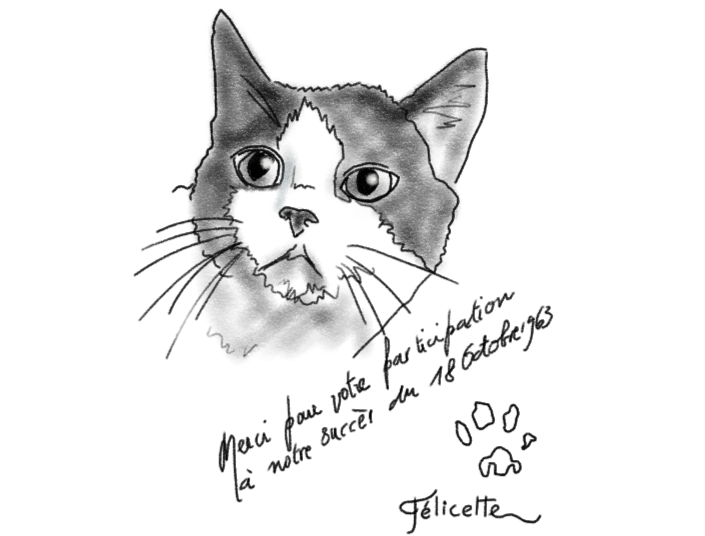
\includegraphics[width=1\linewidth]{img/felicette.png}
    \label{fig:felicette}
\end{figure}


In case you don't know her story, it's worth learning about F\'{e}licette, the first cat in space, who was, perhaps apocryphally, nabbed off the streets of Paris, where she was living happily enough as a stray. She became France's first astronomical envoy and was the only cat to ever cross the K\'{a}rm\'{a}n line. Despite surviving her ordeal and returning to Earth unharmed, she eventually gave her life for science, when she was euthanized to allow French scientists to better study the effects of her trip to space. She is now memorialized with a statue at the International Space University in Strasbourg, France.

The phrase under her portrait translates to ``Thank you for your participation in our success on October 18, 1963.''